%\addcontentsline{toc}{chapter}{Development Process}
\chapter{Design}

\textit{You should concentrate on the more important aspects of the design. It is essential that an overview is presented before going into detail. As well as describing the design adopted it must also explain what other designs were considered and why they were rejected.\\
The design should describe what you expected to do, and might also explain areas that you had to revise after some investigation.\\
Typically, for an object-oriented design, the discussion will focus on the choice of objects and classes and the allocation of methods to classes. The use made of reusable components should be described and their source referenced. Particularly important decisions concerning data structures usually affect the architecture of a system and so should be described here.\\
How much material you include on detailed design and implementation will depend very much on the nature of the project. It should not be padded out. Think about the significant aspects of your system. For example, describe the design of the user interface if it is a critical aspect of your system, or provide detail about methods and data structures that are not trivial. Do not spend time on long lists of trivial items and repetitive descriptions. If in doubt about what is appropriate, speak to your supervisor.\\
You should also identify any support tools that you used. You should discuss your choice of implementation tools - programming language, compilers, database management system, program development environment, etc. \\
Some example sub-sections may be as follows, but the specific sections are for you to define.}

The design for the system was completed in two major steps. First, the initial design was created before any development and following this, incremental changes were made to add  more detail to the design with every relevant feature. The initial design formed the overall model for the system, and was only added to over the duration of the project. The UML class diagrams were designed to be basic initially and only contained major functions and classes. These then evolved as the features were developed.

At the plan by feature level, design was performed at the start of each feature. The feature would be analysed and the relevant functions and variables that were required would be added to the design first. Following this, unit (or system) tests would be designed to exercise the functions as well as the full requirements of the feature.


\section{Informing the Overall model}
\subsection{Use case}
\begin{figure}[h!]
	\centering{
		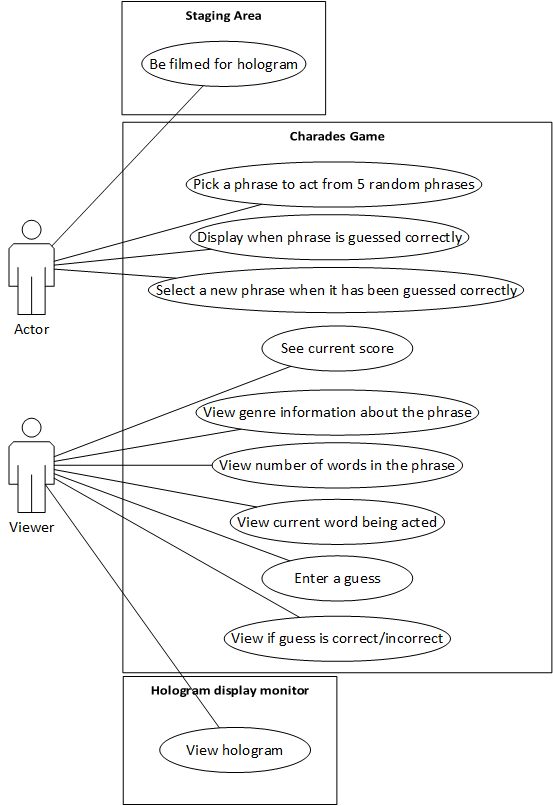
\includegraphics[scale=0.75]{Chapter2/use_case.png}
		\caption{A use case diagram produced to show how the users will interact with the system and the functionality they require.}
		\label{fig:use_case}
	}
\end{figure}
To best identify the requirements of the users, the use case diagram (Figure \ref{fig:use_case}) was produced. In addition to the functionality required by each type of user (Actors and Viewers) the diagram also divides the system into basic subsections. This diagram was a good first step in the early development of the system as it gave an overview of the system as a whole before any major implementation choices were required. Whilst very basic, it also showed interaction with the system that the users would require and acted as the base for the input and output requirements to be address in the user interface design. In addition, the use case diagram showed that the Charades game functionality was dependant on the type of user interacting with the system, which promoted an model-view-controller design pattern to be used.

\newpage

\subsection{Activity diagram}
\begin{figure}[h!]
	\centering{
		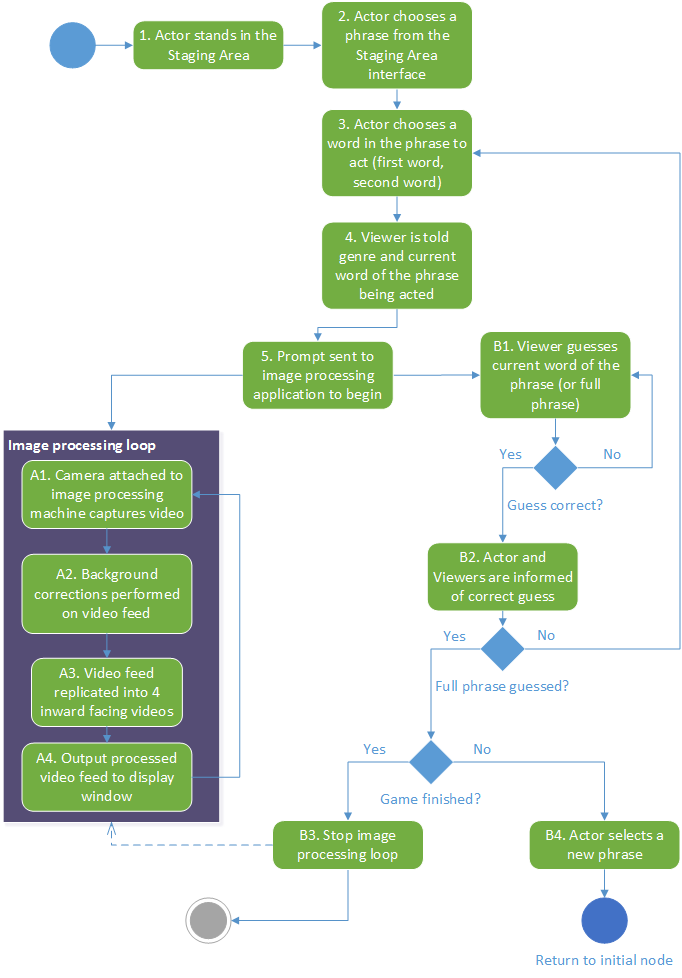
\includegraphics[scale=0.70]{Chapter2/activity_diagram.png}
		\caption{An activity diagram that describes the flow of information in the system. Includes the data flow for both the Hologram and Charades systems.}
		\label{fig:activity_diagram}
	}
\end{figure}
Given the system was deigned to be a game of charades, it follows a linear set of instructions that mirror the original rules of the charades game. An activity diagram was chosen to model the flow of activities in the system due to the well defined path of game play. Figure \ref{fig:activity_diagram} shows an activity diagram that maps the basic flow of a single round of the game. The \textit{Image processing loop}, shown in purple, describes the flow  of the hologram creation. This process (prefixed with the letter A) run continuously in parallel with the game loop (prefixed with the letter B).

\subsection{Component diagram}
\begin{figure}[h!]
	\centering{
		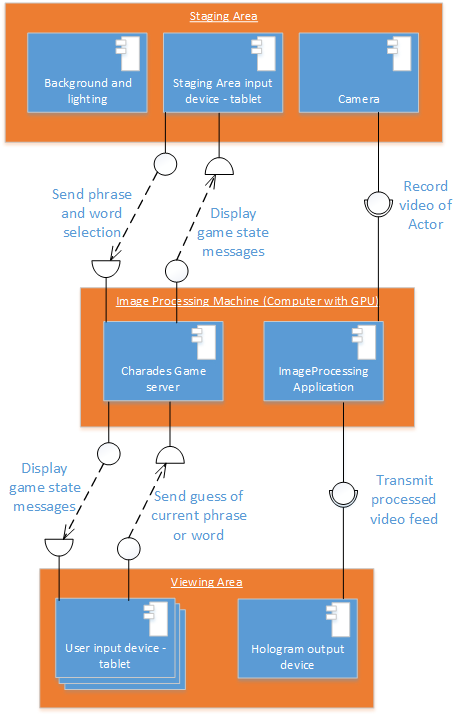
\includegraphics[scale=0.75]{Chapter2/component_diagram.png}
		\caption{A component diagram that describes both the software are hardware components of the system and how they interact with each other.}
		\label{fig:component_diagram}
	}
\end{figure}
The system, in its totality, had to include multiple pieces of hardware to operate. The component diagram, shown in Figure \ref{fig:component_diagram}, helped to combine the different hardware considerations in tandem with the software. Furthermore, the diagram confirmed the presence of three separate areas of the project.

The \textbf{Staging Area} would be where the actor would be filmed. The camera directly connects to the ImageProcessing machine via a usb cable for data transfer. The Staging Area input device will use a wireless connection to send and receive messages from the Charades game server that is hosted on the image processing machine.

The \textbf{Image Processing machine} is a computer that acts as the server for the website as well as running the image processing application for the holograms. Due to the nature of the video feed processing in real-time, the computer will require a Graphical processing unit (GPU). The Image Processing application has input of the raw video feed from the camera in the Staging Area and will process the video and output the result.
The Charades Game server is hosted on the Image processing machine. This component will handle the flow between the users in the Viewing Area and the Actor in the Staging Area.
\section{Overall Architecture}
\subsection{Hologram creation system}

\subsection{Website}

\subsection{UI Design}

\section{Implementation tools}
\subsection{Python}
Python is a free, easy to learn and easy to read programming language. As a scripting language, it offers lightweight solutions to software problems without requiring long compile times. Python, whilst not a fully object orientated (OO) language, provides OO support and this approach is encouraged by the community for larger projects.

\subsection{Pycharm}


\subsection{OpenCV}
OpenCV is an open source software library that provides solutions to common computer vision problems. It is an ideal library for handling image manipulation and offers easy solutions to image display and rendering. OpenCV comes with precompiled binary interfaces for C++, Python, Java and MATLAB and is supported on Windows, Linux, Android and Mac OS \cite{open_cv_binaries}.

\subsection{Django}
Django 